\documentclass{beamer}
\usepackage[english]{babel}
\usepackage{subcaption}
\usepackage{gensymb}
\usepackage{multicol}
\usepackage{natbib}
\usepackage{textcomp}
\useoutertheme{infolines}
\definecolor{vubgreen}{rgb}{0.67,0.698,0.00784} 
\definecolor{vubdarkgreen}{rgb}{0.374,0.373,0.290} 
\definecolor{vubgrey}{rgb}{0.549,0.510,0.431}
\setbeamercolor*{structure}{fg=vubgreen,bg=vubdarkgreen,bg_alt=vubgrey}
\setbeamercolor*{palette primary}{use=structure,fg=white,bg=structure.fg}
\setbeamercolor*{palette secondary}{use=structure,fg=white,bg=structure.fg!75!black}
\setbeamercolor*{palette tertiary}{use=structure,fg=white,bg=structure.fg!50!black}
\setbeamercolor*{palette quaternary}{use=structure,fg=white,bg=structure.bg}
\setbeamercolor*{sidebar}{use=structure,bg=structure.fg}
\setbeamercolor*{palette sidebar primary}{use=structure,fg=structure.fg!10}
\setbeamercolor*{palette sidebar secondary}{fg=white}
\setbeamercolor*{palette sidebar tertiary}{use=structure,fg=structure.fg!50}
\setbeamercolor*{palette sidebar quaternary}{fg=white}
\setbeamercolor*{titlelike}{use=structure,fg=vubgrey,bg=white}
\setbeamercolor*{separation line}{}
\setbeamercolor*{fine separation line}{}
%\newcommand{\Section}[1]{\section{#1} \setcounter{figure}{1}}
\renewcommand{\thefigure}{\thesection.\arabic{figure}}
\setbeamerfont{frametitle}{size={\huge}}
\newcommand{\myitem}{\item[$\bullet$]}
\newcommand{\nireitem}{\item[$\Rightarrow$]}
\makeatletter
\setbeamertemplate{footline}
{
%  \leavevmode%
  \hbox{%
  \begin{beamercolorbox}[wd=.25\paperwidth,ht=2.25ex,dp=1ex,center]{author in head/foot}%
    \usebeamerfont{author in head/foot}\insertshortauthor
  \end{beamercolorbox}%
  \begin{beamercolorbox}[wd=.5\paperwidth,ht=2.25ex,dp=1ex,center]{title in head/foot}%
    \usebeamerfont{title in head/foot}\insertshorttitle
  \end{beamercolorbox}%
  \begin{beamercolorbox}[wd=.25\paperwidth,ht=2.25ex,dp=1ex,center]{date in head/foot}%
    %\usebeamerfont{date in head/foot}\insertshortdate{}\hspace*{2em}
    \insertframenumber /\inserttotalframenumber
  \end{beamercolorbox}}%
%  \vskip0pt%
}
\makeatother

\usepackage{caption}
\captionsetup{labelformat=empty,labelsep=none}
\newcommand\pro{\item[$+$]}
\newcommand\con{\item[\textcolor{red}{$-$}]}

\begin{document}

\setcounter{section}{0}

\title[Real Time Camera Tracking and 3D Reconstruction
Using SDF]{Real Time Camera Tracking and 3D Reconstruction
Using Signed Distance Functions}
\author{Joel Kaiser, Oier Mees}
\begin{frame}
 \begin{center}
\begin{figure}[h]
\centering
\LARGE{Real Time Camera Tracking and 3D Reconstruction
Using Signed Distance Functions}\\
\large{Authors: E. Bylow, J. Sturm, C. Kerl, F. Kahl, D. Cremers}\\
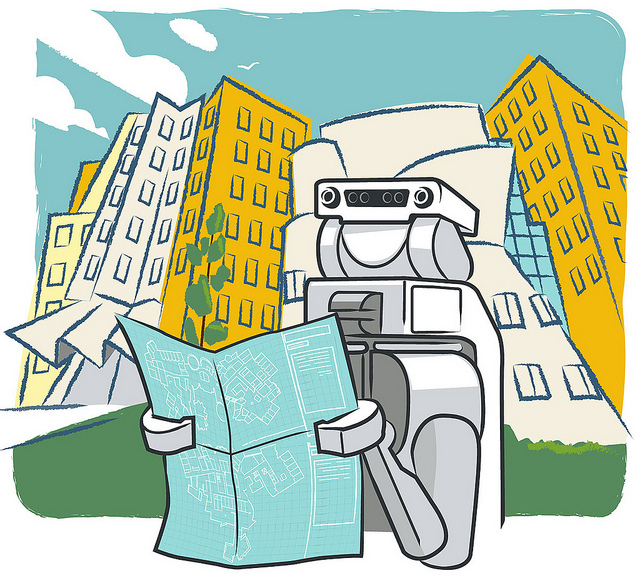
\includegraphics{titleImg.jpg}
\end{figure}
\large{Joel Kaiser, Oier Mees}
\end{center}
\end{frame}


\section{Motivation}
\frame{
\frametitle{Motivation}
3D localization and mapping is fundamental for many robotic applications
\begin{figure}
        \centering
        \captionsetup[subfigure]{labelformat=empty}
                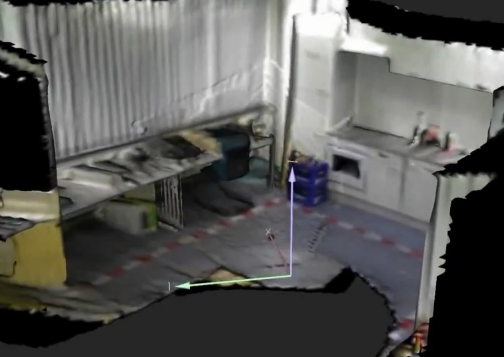
\includegraphics[scale=0.4]{video1.png}
                \caption{\small Source: vision.in.tum.de}
\end{figure}
}
\section{Introduction}
\subsection{Overview}
\frame{
\frametitle{Overview}
\begin{figure}[h]
        \centering
        \captionsetup[subfigure]{labelformat=empty}
                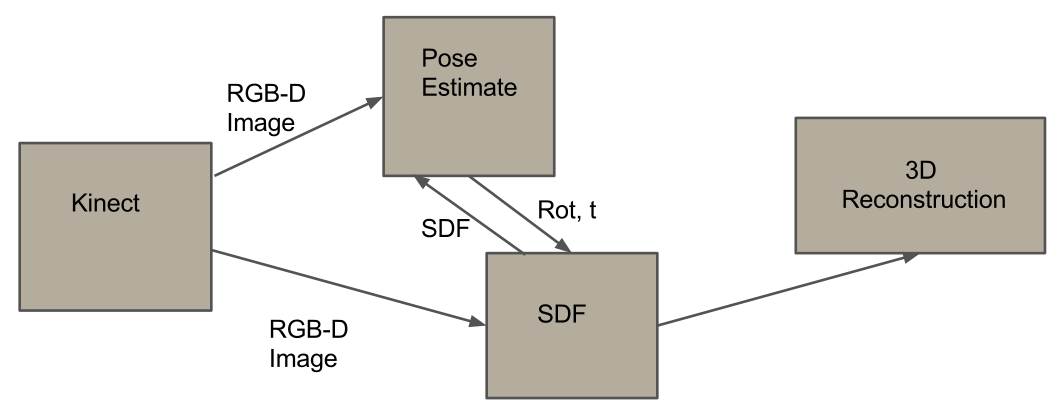
\includegraphics[scale=0.32]{overview.png}
\end{figure}
}

\frame{
\frametitle{Signed Distance Function}
\begin{figure}[h]
        \centering
        \captionsetup[subfigure]{labelformat=empty}
                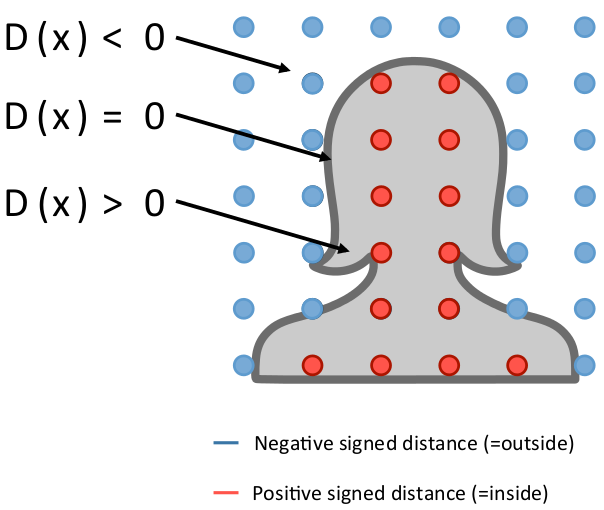
\includegraphics[scale=0.32]{sdf.png}
                \caption{\small Source: lecture "Introduction to Mobile Robotics"}
\end{figure}
}

\frame{
\frametitle{SDF Distances}
\begin{figure}[h]
\vspace*{-30pt}
        \centering
        \captionsetup[subfigure]{labelformat=empty}
                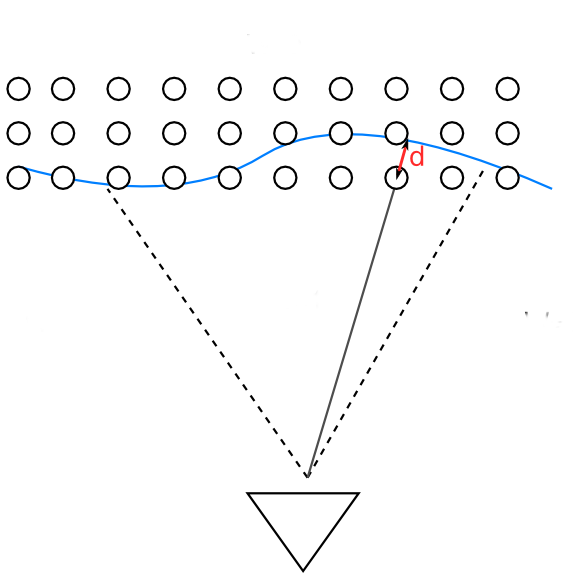
\includegraphics[scale=0.9]{dia_point.png}
                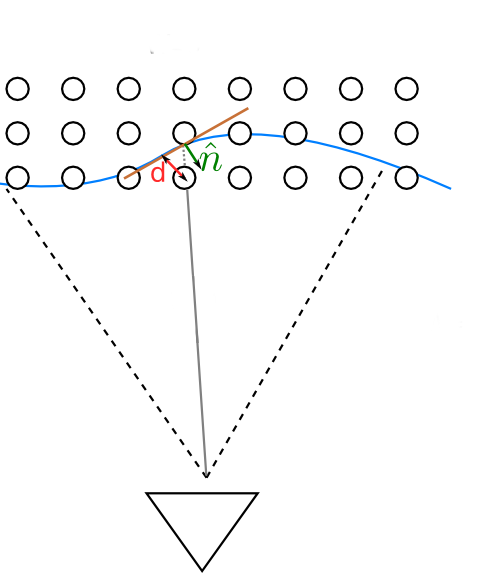
\includegraphics[scale=0.9]{dia_plane2.png}
                \caption{Point-To-Point \hspace*{3cm} Point-To-Plane}
\end{figure}
}
\frame{
\frametitle{SDF Weighting and Truncation}
\begin{figure}[h]
        \centering
        \captionsetup[subfigure]{labelformat=empty}
				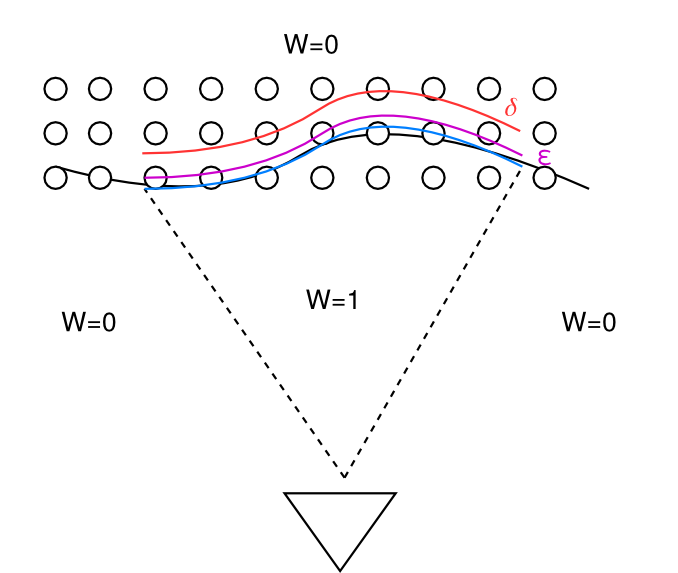
\includegraphics[scale=0.8]{dia1.png}
				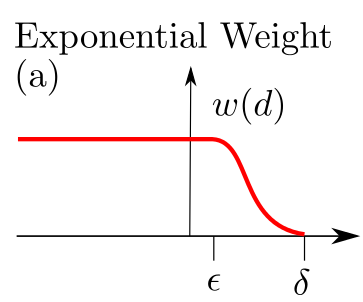
\includegraphics[scale=0.3]{exponential_weight.png}

\end{figure}
}
%\frame{
%\frametitle{Camera Tracking}
%\begin{figure}[h]
%        \centering
%        \captionsetup[subfigure]{labelformat=empty}
%                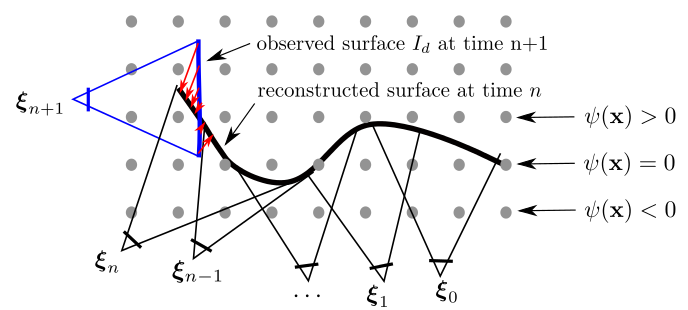
\includegraphics[scale=0.45]{camera.png}
%                \caption{Source: \cite{bylow2013real}}
%\end{figure}
%}





\frame{
\frametitle{3D Reconstruction: Marching Cubes}
\begin{figure}[h]
        \centering
        \captionsetup[subfigure]{labelformat=empty}
                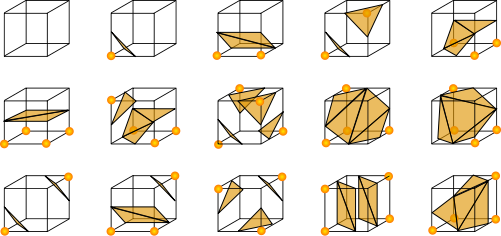
\includegraphics[scale=0.4]{marchingcubes.png}
                \caption{Source: Wikipedia}
\end{figure}
}
\section{Implementation}
\frame{
\frametitle{SDF Reconstruction}
\begin{columns}
		\column{0.4\textwidth} 
			\begin{figure}
				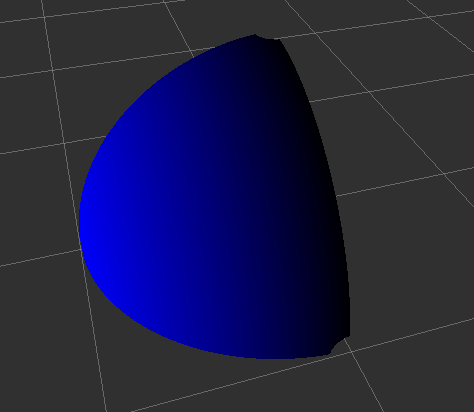
\includegraphics[scale=0.33]{visualization1.png}
			\end{figure}
		\column{0.5\textwidth} 
		%\vspace{-40pt}
			\begin{itemize}
				\item Extended PCL Marching Cubes
\item Draw SDF mesh in Rviz
\item Color Interpolation
			\end{itemize} 
	\end{columns}

}

\frame{
\frametitle{Perception}
\begin{columns}
		\column{0.45\textwidth} 
			\begin{figure}
				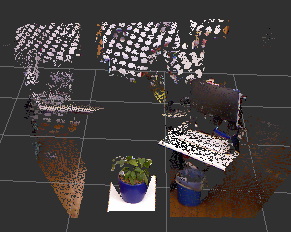
\includegraphics[scale=0.5]{pcl2.png}
			\end{figure}
		\column{0.55\textwidth} 
		%\vspace{-40pt}
			\begin{itemize}
				\item Creating Point Clouds on the fly from RGB and Depth images
				\item Preprocessing for point-to-plane:
				\begin{itemize}
				\item Computing point cloud normals
				\item Applying bilateral filter
				\end{itemize}
				\item Reading trajectory ground truth  with TF
				\item Record Kinect data with rosbag to validate approach
			\end{itemize} 
	\end{columns}

}
%----------------------------------------------------------
%           START CAMERA TRACKING
%----------------------------------------------------------
\frame{
\frametitle{Camera Tracking - What we have}
\begin{columns}
		\column{0.45\textwidth} 
			\begin{figure}
				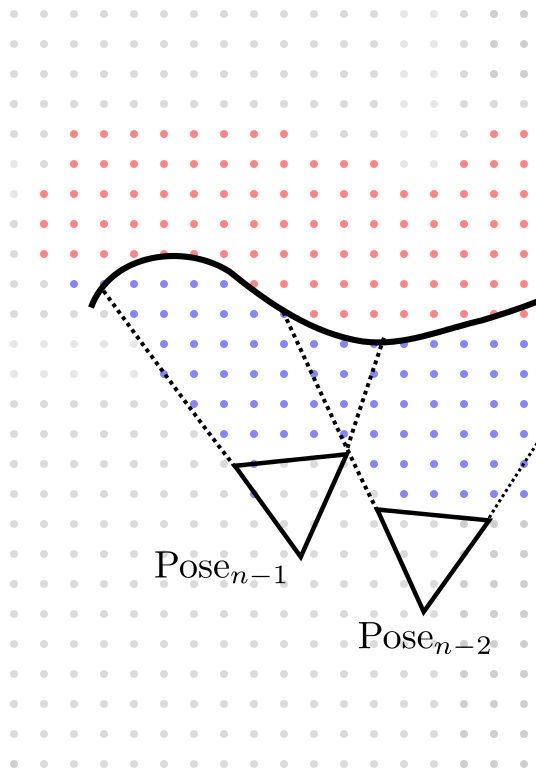
\includegraphics[scale=0.25]{camera_estimation1.png}
			\end{figure}
		\column{0.55\textwidth} 
		%\vspace{-30pt}
		\begin{itemize}
			    \item Successfully estimated our previous camera positions
				%\item Minimize reprojection error with Gauss-Newton using Twist coordinates
				%\item Computation of SDF partial derivatives
				%\item Exponential mapping
		\end{itemize}
\end{columns}
}
\frame{
\frametitle{Camera Tracking - What we get}
\begin{columns}
		\column{0.45\textwidth} 
			\begin{figure}
				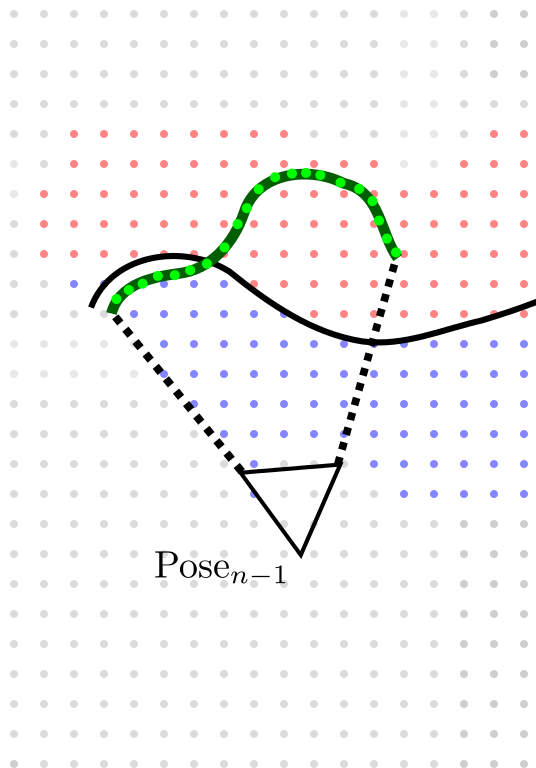
\includegraphics[scale=0.25]{camera_estimation2.png}
			\end{figure}
		\column{0.55\textwidth} 
		%\vspace{-30pt}
			\begin{itemize}
			    \item Successfully estimated our previous camera positions
			    \item New point cloud given by perception
				%\item Minimize reprojection error with Gauss-Newton using Twist coordinates
				%\item Computation of SDF partial derivatives
				%\item Exponential mapping
		\end{itemize}
	\end{columns}
}
\frame{
\frametitle{Camera Tracking - What we want}
\begin{columns}
		\column{0.45\textwidth} 
			\begin{figure}
				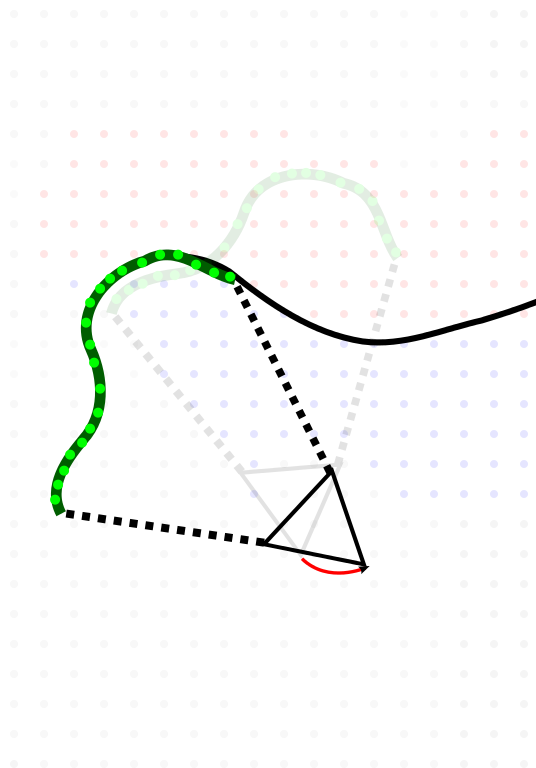
\includegraphics[scale=0.25]{camera_estimation4.png}
			\end{figure}
		\column{0.55\textwidth} 
		%\vspace{-30pt}
			\begin{itemize}
			    \item Successfully estimated our previous camera positions
			    \item New point cloud given by perception
			    \item We search transition from last camera position
				%\item Minimize reprojection error with Gauss-Newton using Twist coordinates
				%\item Computation of SDF partial derivatives
				%\item Exponential mapping
		\end{itemize}
	\end{columns}
}
\frame{
\frametitle{Camera Tracking - What we want}
\begin{columns}
		\column{0.45\textwidth} 
			\begin{figure}
				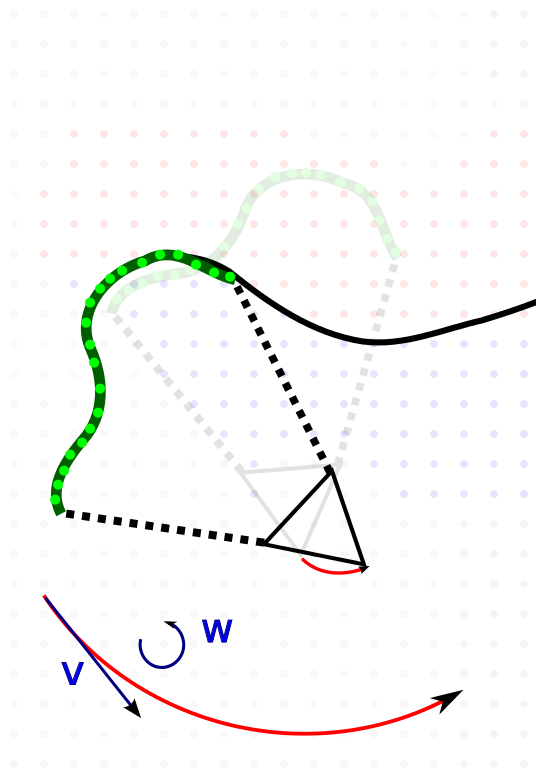
\includegraphics[scale=0.25]{camera_estimation5.png}
			\end{figure}
		\column{0.55\textwidth} 
		%\vspace{-30pt}
			\begin{itemize}
			    \item Successfully estimated our previous camera positions
			    \item New point cloud given by perception
			    \item We search transition from last camera position\\
			    given in twist coordinates $\xi = (\underbrace{v_1, v_2, v_3}_{\text{linear velocity}}, \underbrace{w_1, w_2, w_3}_{\text{angular velocity}})$
				%\item Minimize reprojection error with Gauss-Newton using Twist coordinates
				%\item Computation of SDF partial derivatives
				%\item Exponential mapping
		\end{itemize}
	\end{columns}
}
\frame{
\frametitle{Camera Tracking - How we get it}
\begin{columns}
		\column{0.45\textwidth} 
			\begin{figure}
				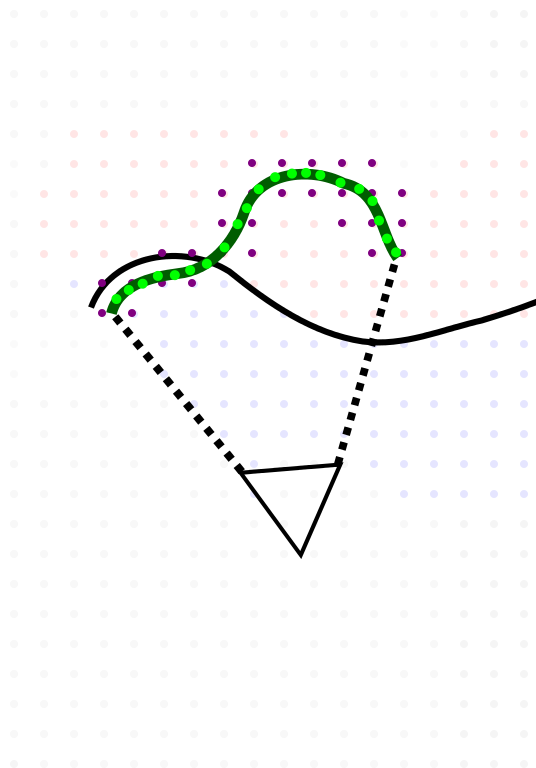
\includegraphics[scale=0.25]{camera_estimation3.png}
			\end{figure}
		\column{0.55\textwidth} 
		%\vspace{-30pt}
			\begin{itemize}
			    \item Successfully estimated our previous camera positions
			    \item New point cloud given by perception
			    \item We search transition from last camera position\\
			    given in twist coordinates $\xi = (\underbrace{v_1, v_2, v_3}_{\text{linear velocity}}, \underbrace{w_1, w_2, w_3}_{\text{angular velocity}})$
			    \item Minimize the error
				%\item Minimize reprojection error with Gauss-Newton using Twist coordinates
				%\item Computation of SDF partial derivatives
				%\item Exponential mapping
		\end{itemize}
	\end{columns}
}
\frame{
\frametitle{SDF}
\begin{columns}
		\column{0.55\textwidth} 
			\begin{figure}
				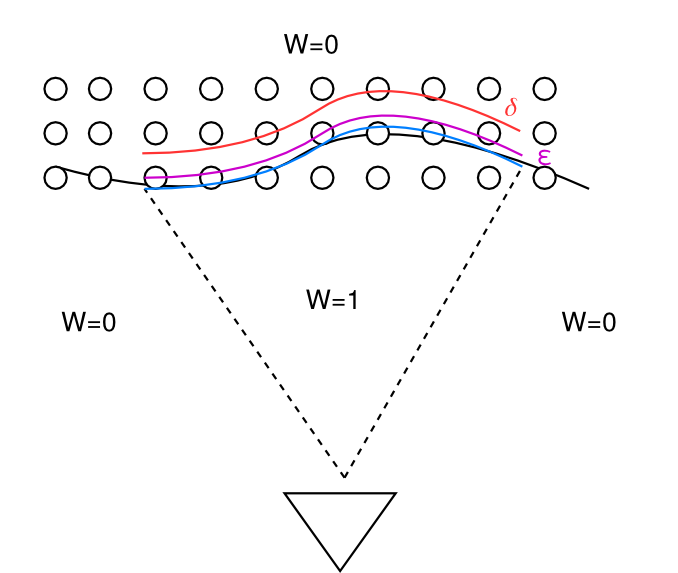
\includegraphics[scale=0.8]{dia1.png}
				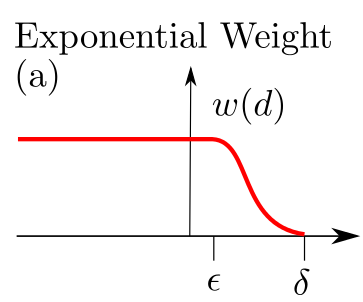
\includegraphics[scale=0.3]{exponential_weight.png}
			\end{figure}
		\column{0.55\textwidth} 
		\vspace{-70pt}
			\begin{itemize}
				\item Implemented Point-to-point and Point-to-plane distances 
				\item Truncation and exponential weighting of distance
		\end{itemize}
	\end{columns}
}

\frame{
\frametitle{Optimizations}

			\begin{itemize}
				\item Extensive use of OpenMP to parallelize:
				\begin{itemize}
				 \item SDF update, Camera Tracking and Marching Cubes
				 \item Initial difficulties due to need to concatenate results
				 \end{itemize} 
				\item Usage of Valgrind profiler to detect bottlenecks and memory leaks
		\end{itemize}

}

\frame{
\frametitle{Live Demo!}
}


\section{Results}

\frame{
\frametitle{Evaluation}

			\begin{itemize}
				\item RGB-D SLAM Dataset and Benchmark online evaluation
		\end{itemize}
		\begin{table}[h]

\centering
\begin{tabular}{|c|c|c|c|c|c|}
\hline
m  & method &  max $\Delta$$\xi$ &  pub rate & trans error& notes\\
\hline
200   & Point-To-Plane& 0.001  & 0.04 & 0.125 m& laptop\\
256  & Point-To-Plane& 0.001  & 1.0 & 0.418 m&desktop\\
256  & Point-To-Plane& 0.001  & 0.1 & 0.060 m&\\
256  & Point-To-Plane& 0.0001  & 0.1 & 0.060 m&\\
512 & Point-To-Plane & 0.01 &  0.1 & 0.320 m &\\
512  & Point-To-Plane& 0.001  & 0.1 & 0.071 m & out of memory\\
256  & Point-To-Plane& 0.001  & 0.1 & 0.060 m & gram schmidt\\
256  & Point-To-Point& 0.001  & 0.1 & \textbf{0.057 m} & \\
\hline
256 & Point-To-Point&  & & 0.047 m & Paper\\
\hline
\end{tabular}
\caption{$\delta$$=0.3m$, $\epsilon$$=0.025$, Gauss-Newton every 9th pixel, RMSE absolute translational error }
\end{table}

}
\frame{
\frametitle{Results}
\begin{figure}[h]
\centering
 \begin{subfigure}[h]{0.5\textwidth}
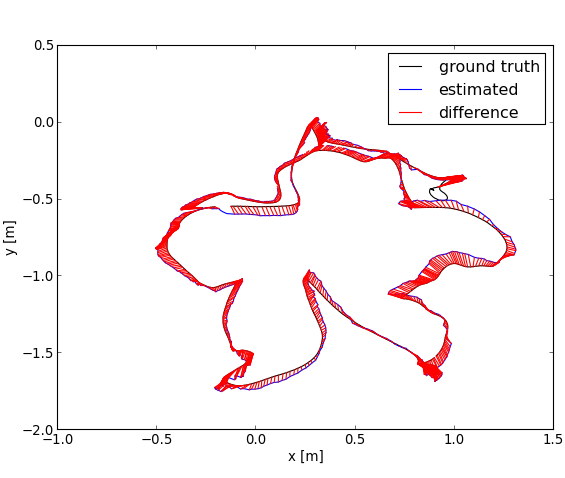
\includegraphics[scale=0.34]{absolute_trajectory_error_best.png}
\caption{Our best result, 0.057 m error}
 \end{subfigure}
 %\qquad
                \begin{subfigure}[h]{0.49\textwidth}
                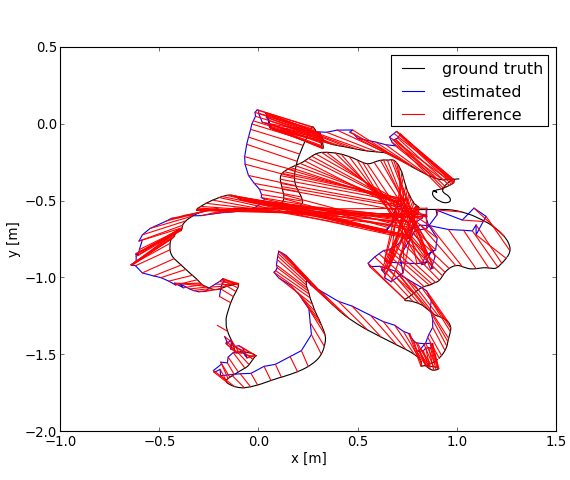
\includegraphics[scale=0.345]{absolute_trajectory_error_worst.png}
                \caption{1.0 publish rate, 0.418 m error }
        \end{subfigure}
\end{figure}

}




\newcommand{\deftitlebar}[5]{\pgfdeclarehorizontalshading{frametitlebarhshad}{#1}{color(#2)=(#3); color(#4)=(#5)}}
\deftitlebar{0.01\paperheight}{0\paperwidth}{olive}{\the\paperwidth}{white} % can be changed during the presentation
\setbeamertemplate{frametitle}
{
	\hspace*{-0.035\paperwidth} \vbox{\insertframetitle}\par
	\hspace*{-0.045\paperwidth}\pgfuseshading{frametitlebarhshad}
}

\begin{frame}
\frametitle{\centerline{QA}}
\begin{figure}[h]
\centering

\includegraphics[scale=0.3]{QA.jpg}
\end{figure}
\end{frame}

\section{Bibliography}
%\clearpage
\begin{frame}[allowframebreaks]
\frametitle{Bibliography}
\small
\bibliographystyle{plainnat}
%\nocite{*}
\bibliography{bibliography}
\vspace*{0.5cm}
Th title image page is by Josh Ellingson and available under Creative Commons (NC, BA) license at \url{www.flickr.com/photos/willowgarage}.
\end{frame}



\end{document}
